% !TeX spellcheck = en_US

%!TEX root = ../thesis.tex
%*******************************************************************************
%****************************** Second Chapter *********************************
%*******************************************************************************

\newcommand{\ba}{\mathbf{a}}
\newcommand{\bb}{\mathbf{b}}
%\newcommand{\bd}{\mathbf{d}}
\newcommand{\bw}{\mathbf{w}}
\newcommand{\bx}{\mathbf{x}}
\newcommand{\by}{\mathbf{y}}
\newcommand{\Exp}[2]{\mathbb{E}_{#1}\left[#2\right]}
\newcommand{\Var}[2]{\text{Var}_{#1}\left[#2\right]}
\newcommand{\Cov}[2]{\text{Cov}_{#1}\left[#2\right]}
\newcommand{\Corr}[2]{\text{Corr}_{#1}\left[#2\right]}

\newcommand{\bA}{\mathbf{A}}
\newcommand{\bB}{\mathbf{B}}
\newcommand{\bV}{\mathbf{V}}
\newcommand{\bW}{\mathbf{W}}
\newcommand{\bv}{\mathbf{v}}

\newcommand{\bphi}{\mathbf{\phi}}
\newcommand{\bt}{\mathbf{\theta}}
\newcommand{\bdelta}{\mathbf{\delta}}
\newcommand{\beps}{\mathbf{\epsilon}}
\newcommand{\q}{q_\mathbf{\phi}}
\newcommand{\bmu}{\mathbf{\mu}}
\newcommand{\bsigma}{\mathbf{\sigma}}
\newcommand{\bSigma}{\mathbf{\Sigma}}

\newcommand{\D}{\mathcal{D}}

\newcommand{\eqnr}{\addtocounter{equation}{1}\tag{\theequation}}

\chapter{Kiến thức chuẩn bị}

\ifpdf
\graphicspath{{Chapter2/Figs/Raster/}{Chapter2/Figs/PDF/}{Chapter2/Figs/}}
\else
\graphicspath{{Chapter2/Figs/Vector/}{Chapter2/Figs/}}
\fi


\pagebreak

\section{Neural Networks}
\subsection{Brain Analogies}

Theo Rosenblatt, một nhà tâm lý học nổi tiếng, tri giác (perceptron) được hình thành như một mô hình toán học về cách mà những tế bào thần kinh (neural) hoạt động trong bộ não của chúng ta. Theo Rosenblatt, một neural nhận một bộ đầu vào nhị phân (từ những neuron gần trước đó), nhân mỗi đầu vào với một trọng số nhất định rồi lấy tổng. Nếu tổng thu được đủ lớn thì đầu ra sẽ là 1, ngược lại là 0 (cách neuron chọn lọc những thông tin quan trọng)

\begin{figure}[h]
	\begin{center}
		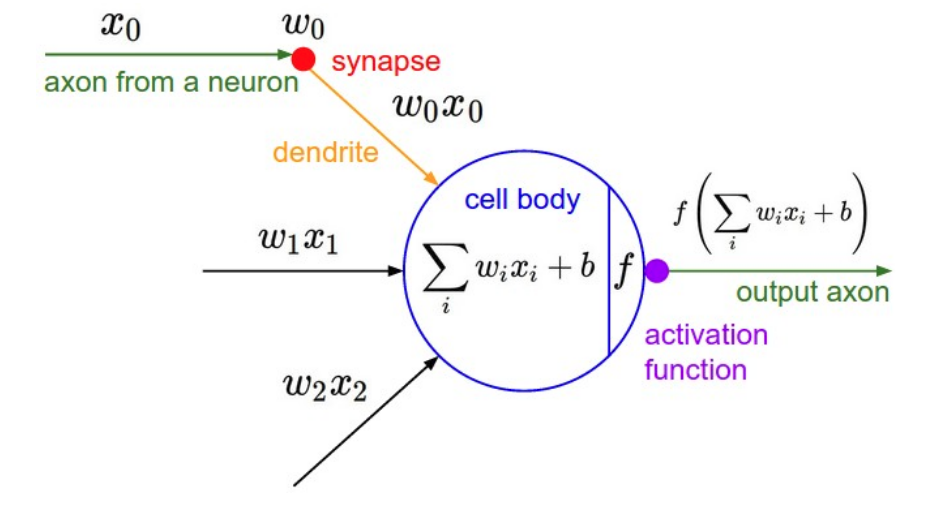
\includegraphics[height=.28\textheight]{Chuong2/Figs/NeuralNetwork.png}
		\label{fig:Neural_Network}
		\caption{Biologically inspired Neural Network \cite{karparthy}}
	\end{center}
\end{figure}

\subsection{Mạng lưới thần kinh nhân tạo}
Lấy ý tưởng từ mạng lưới thần kinh sinh học, cấu trúc của mạng lưới thần kinh nhân tạo (Neural Network: NN) được phát triển để xử lý thông tin tương tự cách bộ não xử lý thông tin. Một khối lượng lớn các quy trình kết nối các phần tử (neural) làm việc cùng nhau làm cho NN có thể giải quyết các vấn đề phức tạp. Giống như con người học từ các ví dụ, NN cũng vậy. Việc học trong hệ thống sinh học là những điều chỉnh các kết nối khớp thần kinh (synaptic) tương tự như việc cập nhật các trọng số trong NN.
Một NN bao gồm 3 lớp: lớp đầu vào (input layer) nơi tiếp nhận dữ liệu, lớp ẩn (hidden layer) để học hỏi cách biểu diễn dữ liệu hợp lý và lớp đầu ra (output) để đưa ra kết quả, dự đoán.Mạng nơ-ron có thể được coi là hệ thống từ đầu đến cuối để tìm ra các đặc trưng trong dữ liệu quá phức tạp để con người có thể nhận ra để dạy cho máy.
\begin{figure}[h]
	\begin{center}
		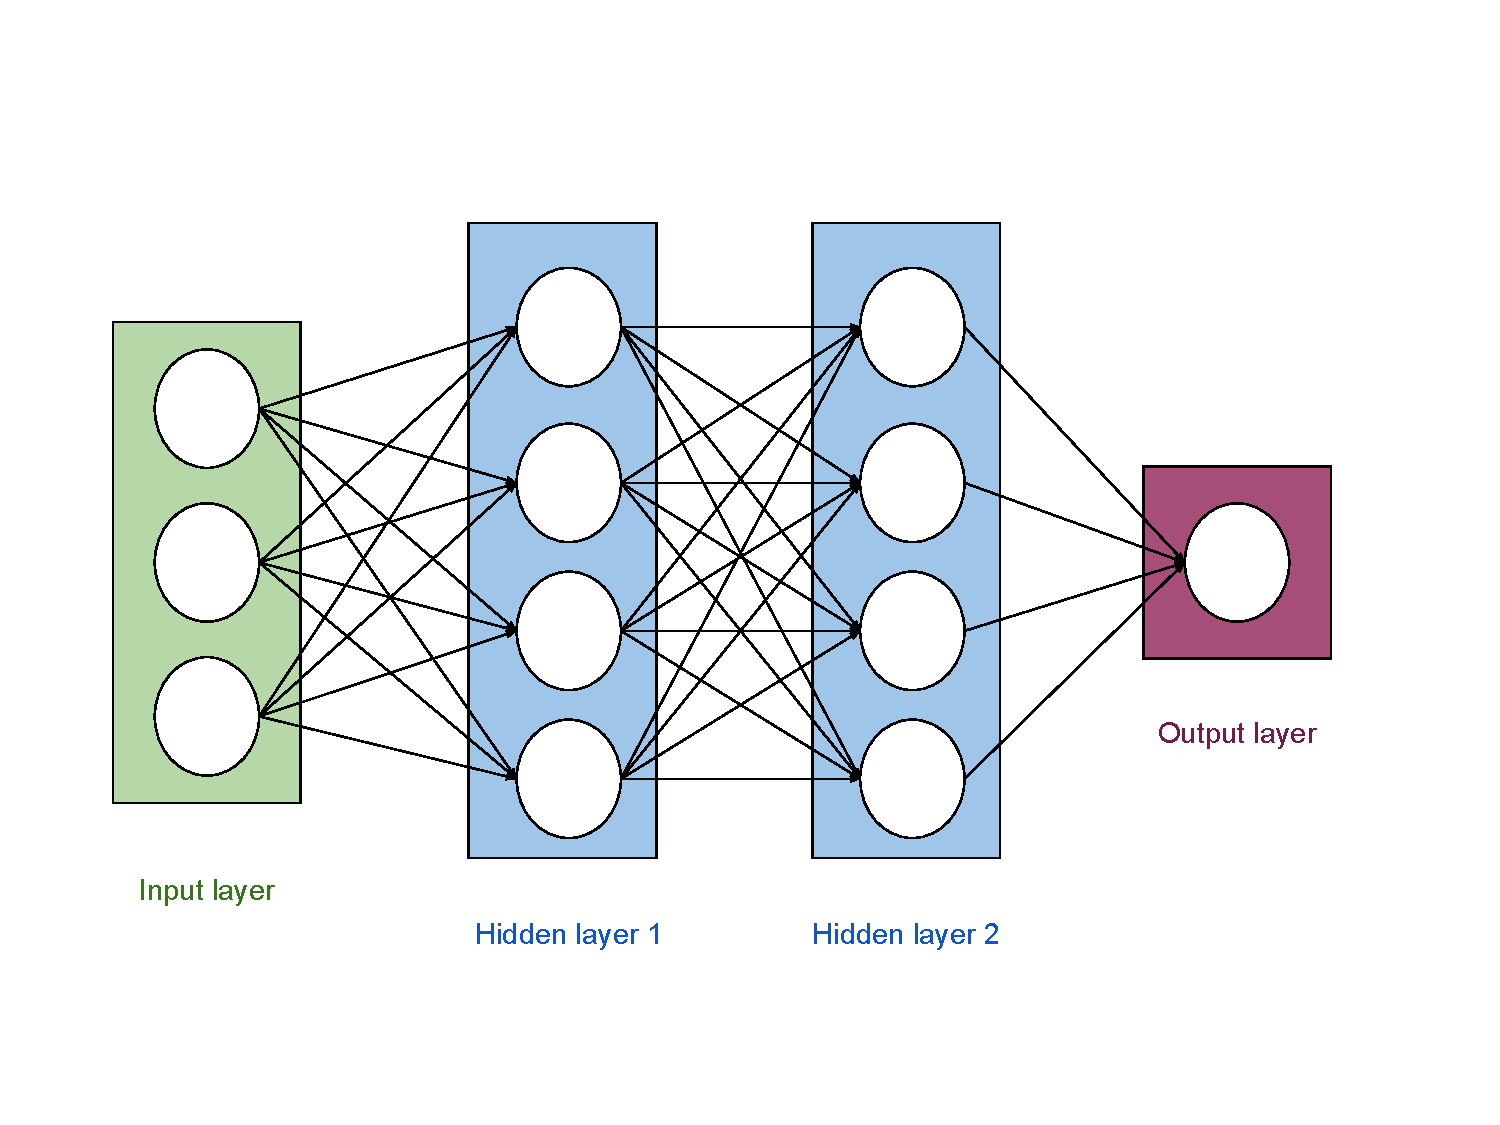
\includegraphics[height=.58\textheight]{Chuong2/Figs/MLP.pdf}
		\label{fig:Two Layered Neural Network}
		\caption{MLP với hai lớp ẩn}
	\end{center}
\end{figure}

\subsubsection{Multi-layer Perceptron (MLP)}
Multi-layer Perceptron (MLP) là dạng đơn giản NN, ta đi qua các khái niệm và ký hiệu:
\begin{enumerate}
	\item Lớp (Layer): Ngoài lớp đầu vào và lớp đầu ra, một MLP có thể có nhiều lớp ẩn (hidden layers) ở giữa. Các lớp ẩn theo thứ tự từ đầu vào đến đầu ra được đánh số thứ tự là Hidden layer 1, Hidden layer 2, ... Hình \eqref{fig:Two Layered Neural Network} là một ví dụ về MLP với 2 lớp ẩn
	\item Units: Một node hình tròn trong một lớp gọi là unit. Unit ở các lớp đầu vào, lớp ẩn và lớp đầu ra. Đầu vào của các lớp ẩn được ký hiệu bỡi $\textit{z}$, đầu ra của mỗi unit thường được ký hiệu bằng $\textit{a}$ (thể hiện hàm activation, tức là giá trị của mỗi unit sau khi ta áp dụng hàm activation). Đầu ra của unit thứ \textit{i} được ký hiệu là $a_{i}^{(l)}$. Giả sử thêm rằng số unit trong lớp thứ $(l)$ là $d^{(l)}$. Vector biểu diễn đầu ra của lớp $l$ được ký hiệu là $\textbf{a}^{(l)}\in \mathbb{R}^{d^{(l)}}$.
	\begin{figure}[h]
		\begin{center}
			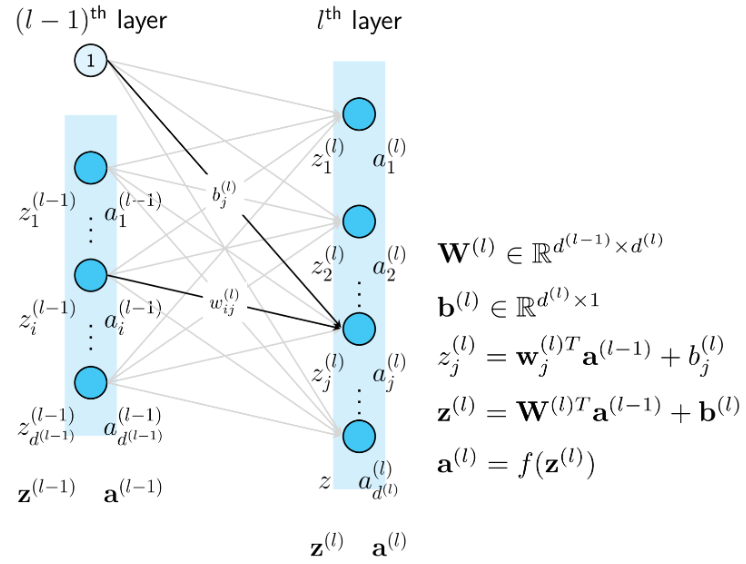
\includegraphics[height=.58\textheight]{Chuong2/Figs/kyhieu.png}
			\label{fig:ky hieu trong MLP}
			\caption{Các ký hiệu sử dụng trong MLP.}
		\end{center}
	\end{figure}
	\item Trọng số và Độ lệch (Weight and Bias): Có $\textbf{L}$ ma trận trọng số cho một MLP có $\textbf{L}$ lớp. Các ma trận này được ký hiệu là $\textbf{W}^{(l)} \in \mathbb{R}^{d^{(l-1)} \times d^{(l)}},l = 1,2,...,L$ trong đó $\textbf{W}^{(l)}$ thể hiện kết nối từ lớp thứ $l=1$ tới lớp thứ $l$ (nếu ta coi lớp đầu vào là lớp 0). Cụ thể hơn, phần tử $w_{ij}^{(l)}$ thể hiện kết nối từ node thứ $i$ của lớp thứ $(l-1)$ tới node thứ $j$ của lớp thứ $(L)$. Các biases của lớp thứ $(l)$ được ký hiệu là $\textbf{b}^{(L)}\in \mathbb{R}^{d^{(l)}}$. Các trọng số này được ký hiệu như trên \ref{fig:ky hieu trong MLP}. Khi tối ưu một MLP cho một công việc nào đó, chúng ta cần tìm các trọng số và biases này. Tập hợp các trọng số và biases lần lượt được ký hiện là $\textbf{W}$ và $\textbf{b}$.
	\item Các hàm kích hoạt (Activation Functions): Mỗi đầu ra của một unit được tính dựa vào công thức:
	\begin{equation}
	a_{i}^{(l)} = f(\textbf{w}_{i}^{(l)T}a^{(l-1)}+b_{i}^{(l)})
	\end{equation}
	Trong đó $f(.)$ là một (không tuyến tính: nonlinear) hàm kích hoạt. Ở dạng vector, biểu thức bên trên được viết là:
	\begin{equation}
	a^{(l)} = f(\textbf{W}^{(l)T}a^{(l-1)}+b^{(l)})
	\end{equation}
	Khi hàm kích hoạt $f(.)$ được áp dụng cho một ma trận (hoặc vector), ta hiểu rằng nó được áp dụng cho từng thành phần của ma trận đó. Sau đó các thành phần này được sắp xếp lại đúng theo thứ tự để được một ma trận có kích thước bằng với ma trận đầu vào.
\end{enumerate}
\subsubsection{Lan truyền ngược(Backpropagation)}
Phương pháp phổ biến nhất để tối ưu MLP vẫn là Gradient Descent(GD). Để áp dụng GD, chúng ta cần tính được gradient của hàm mất mát theo từng ma trận trọng số $\textbf{W}^{(l)}$ và vector bias $\textbf{b}^{(l)}$. Trước hết, chúng ta cần tính dự đoán đầu ra $\hat{y}$ với một đầu vào $x$:

\begin{align*}
\textbf{a}^{(0)} &= x \\
\textit{z}_{i}^{(l)} &= \textbf{w}_{i}^{(l)T}a^{(l-1)}+b_{i}^{(l)} \\
\textbf{z}^{(l)} &= \textbf{W}^{(l)T}a^{(l-1)}+b^{(l)}, l = 1,2,...,L \\
a^{(l)} &= f(\textbf{z}^{(l)}), l = 1,2,...,L\\
\hat{\textbf{y}} &= \textbf{a}^{(L)} \\
\end{align*}

Bước này gọi là feedforward vì cách tính toán được thực hiện từ đầu đến cuối của mạng.
Giả sử $\textit{J}(\textbf{W,b,X,Y})$ là hàm mất mát của bài toán, trong đó $\textbf{W,b}$ là tập hơp tất cả các ma trận trọng số giữa các lớp và biases của mỗi lớp. $\textbf{X,Y}$ là cặp dữ liệu huấn luyện với mỗi cột tương ứng với một điểm dữ liệu. Để có thể áp dụng các phương pháp gradient-based (mà Gradient Descent là một ví dụ). chúng ta cần tính được:
\begin{equation*}
\frac{\partial J}{\partial \textbf{W}^{(l)}}; \frac{\partial J}{\partial \textbf{b}^{(l)}}, l = 1,2,...,L
\end{equation*}
Một ví dụ của hàm mất mát là hàm Mean Square Error (MSE) tức là \textit{trung bình của bình phương lỗi}.
\begin{align*}
\textit{J}(\textbf{W,b,X,Y}) &= \frac{1}{N}\sum_{n=1}^{N} \vert\vert \textbf{y}_{n} - \hat{\textbf{y}}_{n} \vert\vert_{2}^2 \\
&= \frac{1}{N}\sum_{n=1}^{N} \vert\vert \textbf{y}_{n} - \textbf{a}_{n}^{(L)} \vert\vert_{2}^2
\end{align*}
Với $N$ là số cặp dữ liệu $(\textbf{x,y})$ trong tập huấn luyện.

Việc tính toán trực tiếp giá trị này rất phức tạp vè hàm mất mát không phụ thuộc trực tiếp vào các hệ số. Phương pháp phổ biến nhất được dùng có thể là Backpropagation giúp tính gradient từ llopws cuối cùng đến lớp đầu tiên. Lớp cuối cùng được tính toán trước vì nó gần gũi hơn với đầu ra của mô hình và hàm mất mát. Việc tính toán gradient của các lớp trước được thực hiện dựa trên quy tắc đạo hàm của hàm hợp.

Đạo hàm của hàm mất mát theo chỉ một thành phần của ma trận trọng số của lớp cuối cùng:
\begin{align*}
\frac{\partial J}{\partial w_{ij}^{(L)}} &= \frac{\partial J}{\partial z_{j}^{(L)}}.\frac{\partial z_{j}^{(L)}}{\partial w_{ij}^{(L)}} \\
& = e_{j}^{(L)}a_{i}^{(L-1)}
\end{align*}
Trong đó $e_{j}^{(L)} = \frac{\partial J}{\partial z_{j}^{(L)}}$ thường là một đại lượng dễ tính toán và $\frac{\partial z_{j}^{(L)}}{\partial w_{ij}^{(L)}} = a_{i}^{(L-1)}$ vì $z_{j}^{(L)} = \textbf{w}_{j}^{(L)T}\textbf{a}^{(L-1)}+b_{j}^{(L)}$.
Tương tự như thế, đạo hàm của hàm mất mát theo bias của lớp cuối cùng là:
\begin{equation*}
\frac{\partial J}{\partial b_{j}^{(L)}} = \frac{\partial J}{\partial z_{j}^{(L)}}.\frac{\partial z_{j}^{(L)}}{\partial b_{j}^{(L)}} \\
 = e_{j}^{(L)}
\end{equation*}
\begin{figure}[h]
	\begin{center}
		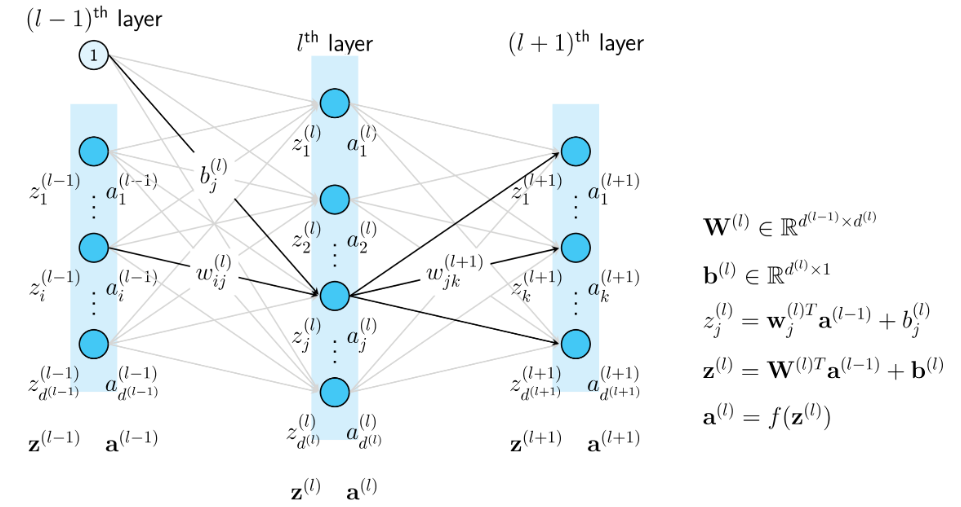
\includegraphics[height=.40\textheight]{Chuong2/Figs/backpropagation.png}
		\label{fig: Mo phong cach tinh backpropagation}
		\caption{Mô phỏng cách tính backpropagation.}
	\end{center}
\end{figure}
Dựa vào hình trên, ta có thể tính được:
\begin{align*}
\frac{\partial J}{\partial w_{ij}^{(l)}} &= \frac{\partial J}{\partial z_{j}^{(l)}}.\frac{\partial z_{j}^{(l)}}{\partial w_{ij}^{(l)}} \\
& = e_{j}^{(l)}a_{i}^{(l-1)}
\end{align*}
với:
\begin{align*}
e_{j}^{(l)} &= \frac{\partial J}{\partial z_{j}^{(l)}}= \frac{\partial J}{\partial a_{j}^{(l)}}.\frac{\partial a_{j}^{(l)}}{\partial z_{j}^{(l)}}\\
& = (\sum_{k=1}^{d^{(l+1)}}\frac{\partial J}{\partial z_{k}^{(l+1)}}.\frac{\partial z_{k}^{(l+1)}}{\partial a_{j}^{(l)}})f^{'}(z_{j}^{(l)})\\
& = (\sum_{k=1}^{d^{(l+1)}}e_{k}^{(l+1)}w_{jk}^{(l+1)})f^{'}(z_{j}^{(l)})\\
& = (\textbf{w}_j^{(l+1)}\textbf{e}^{(l+1)})f^{'}(z_{j}^{(l)})
\end{align*}
trong đó $\textbf{e}^{(l+1)}=[e_{1}^{(l+1)},e_{2}^{(l+1)},...,e_{d^{(l+1)}}^{(l+1)}]^T \in \mathbb{R}^{d^{(l+1)}\time 1}$ và $\textbf{w}_{j:}^{(l+1)}$ được hiểu là hàng thứ \textit{j} của ma trận $\textbf{W}^{(l+1)}$
Với cách làm tương tự, ta có thể suy ra:
\begin{equation*}
\frac{\partial J}{\partial b_{j}^{(l)}} = e_j^{(l)}
\end{equation*}
Nhận thấy rằng trong các công thức trên đây, việc tính $e_j^{(l)}$ đóng một vai trò quan trọng, Hơn nữa, để tính được các giá trị này, ta cần tính được các $e_j^{(l+1)}$. Nói cách khác, ta cần tính ngược các giá trị này từ cuối.
\subsubsection{Convolutional Neural Network}

Vấn đề chính của lớp FC là cần quá nhiều trọng số, làm khối lượng của mô hình lớn đối mặt với những vẫn đề như thời gian đào tạo (training) và đưa ra dự đoán của mô hình chậm và đặc biệt dễ bị overfitting,...
Ví dụ: trọng nhiệm vụ phân loại ảnh, đầu vào là một ảnh có kích thước $64\times64\times3$, FC cần 12288 trọng số cho một đầu ra trong lớp ẩn đầu tiên. Số lượng trọng số sẽ tăng lên rất nhiều lần khi kích thước ảnh tăng.
Ngoài ra, lớp FC còn làm mất thông tin hình học của bức ảnh vì đang xem các điểm ảnh (pixel) độc lập với nhau. Nhưng trong thực tế, các pixel trong từng vùng nhỏ (local) có ảnh hưởng đến nhau. 
Convolutional Neural Network(CNN) được thiết kế ra để giải quyết các vấn đề của FC trong phân loại ảnh.
CNN thường bao gồm các thành phần sau:
\begin{enumerate}
	\item Lớp đầu vào: một ảnh RGB có kích thước $H \times W \times 3$  tương ứng $Height \times Width \times Chanels$.
	\item Khối convolution: bao gồm
	\begin{enumerate}
		\item Lớp convolution: sử dụng một ma trận lọc (kernel hoặc fillters) có kích thước nhỏ, thường là $3\times 3$ hoặc $5\times5$, trượt qua lần lượt khắp ảnh hoặc bản đồ đặc trưng (feature map), thực hiện phép nhân tích chập cho kernel và một phần nhỏ cùng kích thước với kernel trên ảnh, tổng của ma trận tích vừa thu được được xem như một phần tử đầu ra tương ứng trên lớp đó.
		\begin{figure}[h]
			\begin{center}
				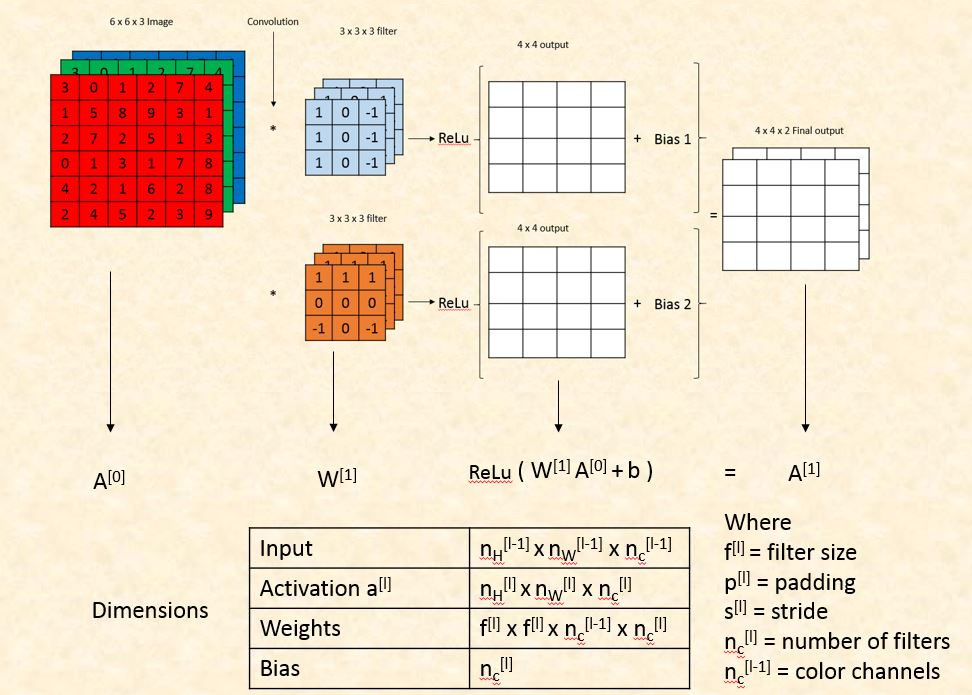
\includegraphics[height=.28\textheight]{Chuong2/Figs/Convolution-Layer-Dimensions.jpg}
				\label{fig:convolution layer}
				\caption{Kích thước tham số của lớp convolution \cite{karparthy}}
			\end{center}
		\end{figure}
		\item Hàm kích hoạt (activation function): thường sử dụng hàm ReLU, được mô tả như hàm $max(0,x)$. Có nghĩa là bất kỳ số thực nào bé hơn 0 được chuyển về 0 trong khi những số thực lớn hơn 0 được giữ nguyên giá trị.
		\item Lớp tổng hợp (Pooling layer): lớp pooling được sử dụng để đơn giản hóa thông tin đầu ra, giảm bớt số lượng neuron. Max-pooling được sử dụng phổ biến nhất, nó chọn giá trị lớn nhất trong vùng đầu vào $2\times 2$. Như vậy, qua lớp max-pooling thì số lượng neuron giảm đi phân nửa. Chúng ta có thể thấy rằng max-pooling lọc những đặc trưng yếu, chỉ giữ lại đặc trưng mạnh nhất.
		\begin{figure}[h]
			\begin{center}
				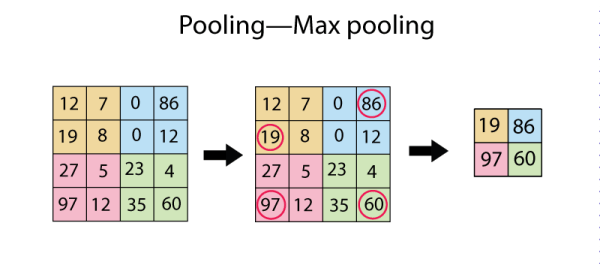
\includegraphics[height=.28\textheight]{Chuong2/Figs/poolingmax.png}
				\label{fig:maxpooling layer}
				\caption{Một ví dụ của lớp max-pooling}
			\end{center}
		\end{figure}
		
	\end{enumerate}
	\item Lớp FC
\end{enumerate}
Trong một mạng CNN, thông thường các lớp được sắp xếp theo thứ tự: lớp đầu vào + một vài khối convolution + lớp FC + lớp đầu ra.
\begin{figure}[h]
	\begin{center}
		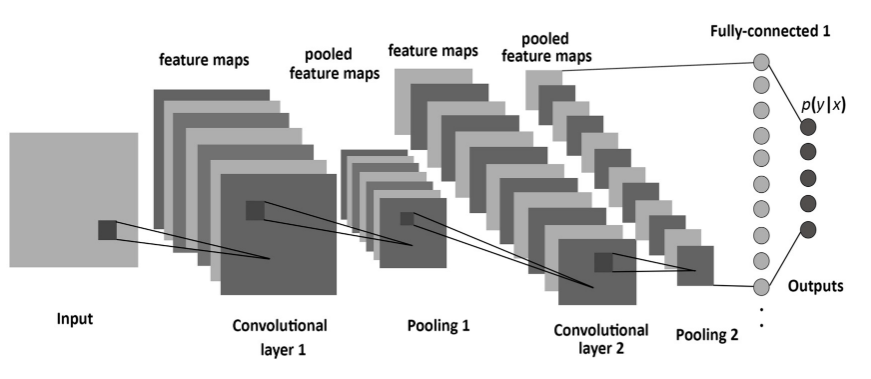
\includegraphics[height=.28\textheight]{Chuong2/Figs/CNN.png}
		\label{fig:CNN}
		\caption{Cấu trúc đầy đủ của một mạng CNN}
	\end{center}
\end{figure}



\section{Khoảng cách giữa hai phân phối}
\subsection{Entropy và cross-entropy}
Entropy là một khái niệm thường gặp trong lý thuyết thông tin. Chúng dùng để đo lượng thông tin mang lại của một sự kiện hay đặc trưng khi biết phân phối xác suất của chúng.
Với một phân phối P,
\begin{equation*}
Entropy = H(P) = \mathbb{E}_{x\sim P}[-logP(x)]
\end{equation*}
Miến là ta biết phân phối xác suất của bất kỳ cái gì, ta đều có thể tính toán entropy của nó.

Trong trường hợp phân phối xác suât thật P ta không biết hoặc rất khó để tính toán, việc tìm được một phân phối Q xấp xỉ P rất có ý nghĩa. Từ đó, ta cần phải định nghĩa một độ đo giữa hai phân phối để có thể đánh giá được việc xấp sỉ P băng Q có hiệu quả hạy chưa?
Ta định nghĩa:
\begin{equation*}
CrossEntropy = H(P,Q) = \mathbb{E}_{x\sim P}[-logQ(x)]
\end{equation*}
CrossEntropy là lượng thông tin mang lại của của sự kiện có phân phối xấp xỉ Q nhưng được lấy mẫu với phân phối thực P.
Lúc này, việc so sánh giữa CrossEntropy và Entropy có ý nghĩa vì chúng đều được lẫy mẫu từ cùng một phân phối.
\subsection{Phân kỳ Kullback-Leibler}
Phân kỳ Kullback-Leibler cho chúng ta biết phân phối Q xấp xỉ phân phối P tốt như thế nào bằng cách tính toán cross-entropy trừ entropy.
\begin{align*}
D_KL(P||Q) &= H(P,Q) - H(P)\\
& = \mathbb{E}_{x\sim P}[-logQ(x)] - \mathbb{E}_{x\sim P}[-logP(x)]\\
& = \mathbb{E}_{x\sim P}[logP(x)-logQ(x)]\\
& = \mathbb{E}_{x\sim P}[log\frac{P(x)}{Q(x)}]
\end{align*}
Phân kỳ KL đo lượng thông tin chênh lệch hay sự không hiệu quá khi sử dụng phân phối Q để xấp xỉ phân phối P.
\begin{figure}[h]
	\begin{center}
		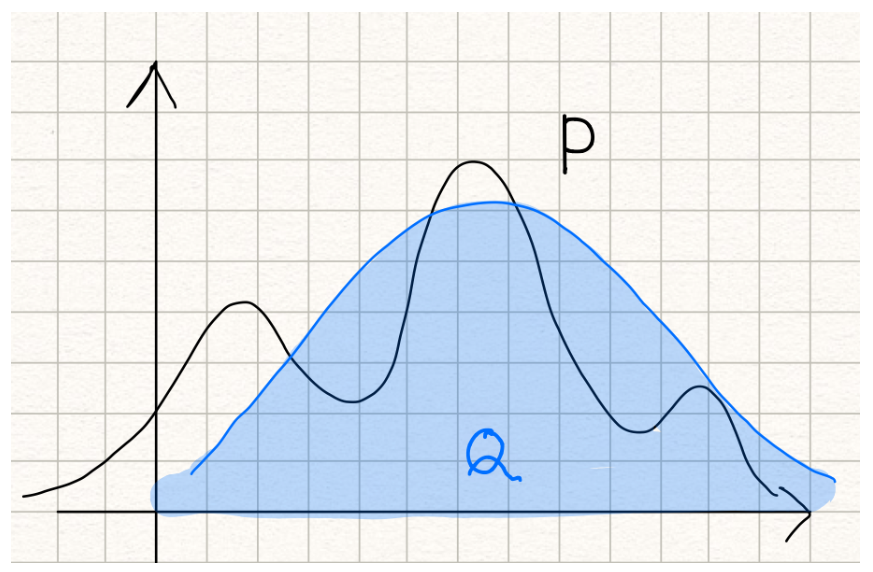
\includegraphics[height=.28\textheight]{Chuong2/Figs/KL.png}
		\label{fig:KL}
		\caption{Xấp xỉ phân phối P bằng Q}
	\end{center}
\end{figure}


